% $Id$

\setcounter{endnote}{0}

%\chapter{Maps}
\label{ch:maps}
\addcontentsline{toc}{chapter}{Maps}

\begin{pspicture}(0,0)(120mm,190mm)
\rput(62.2mm,96.2mm){
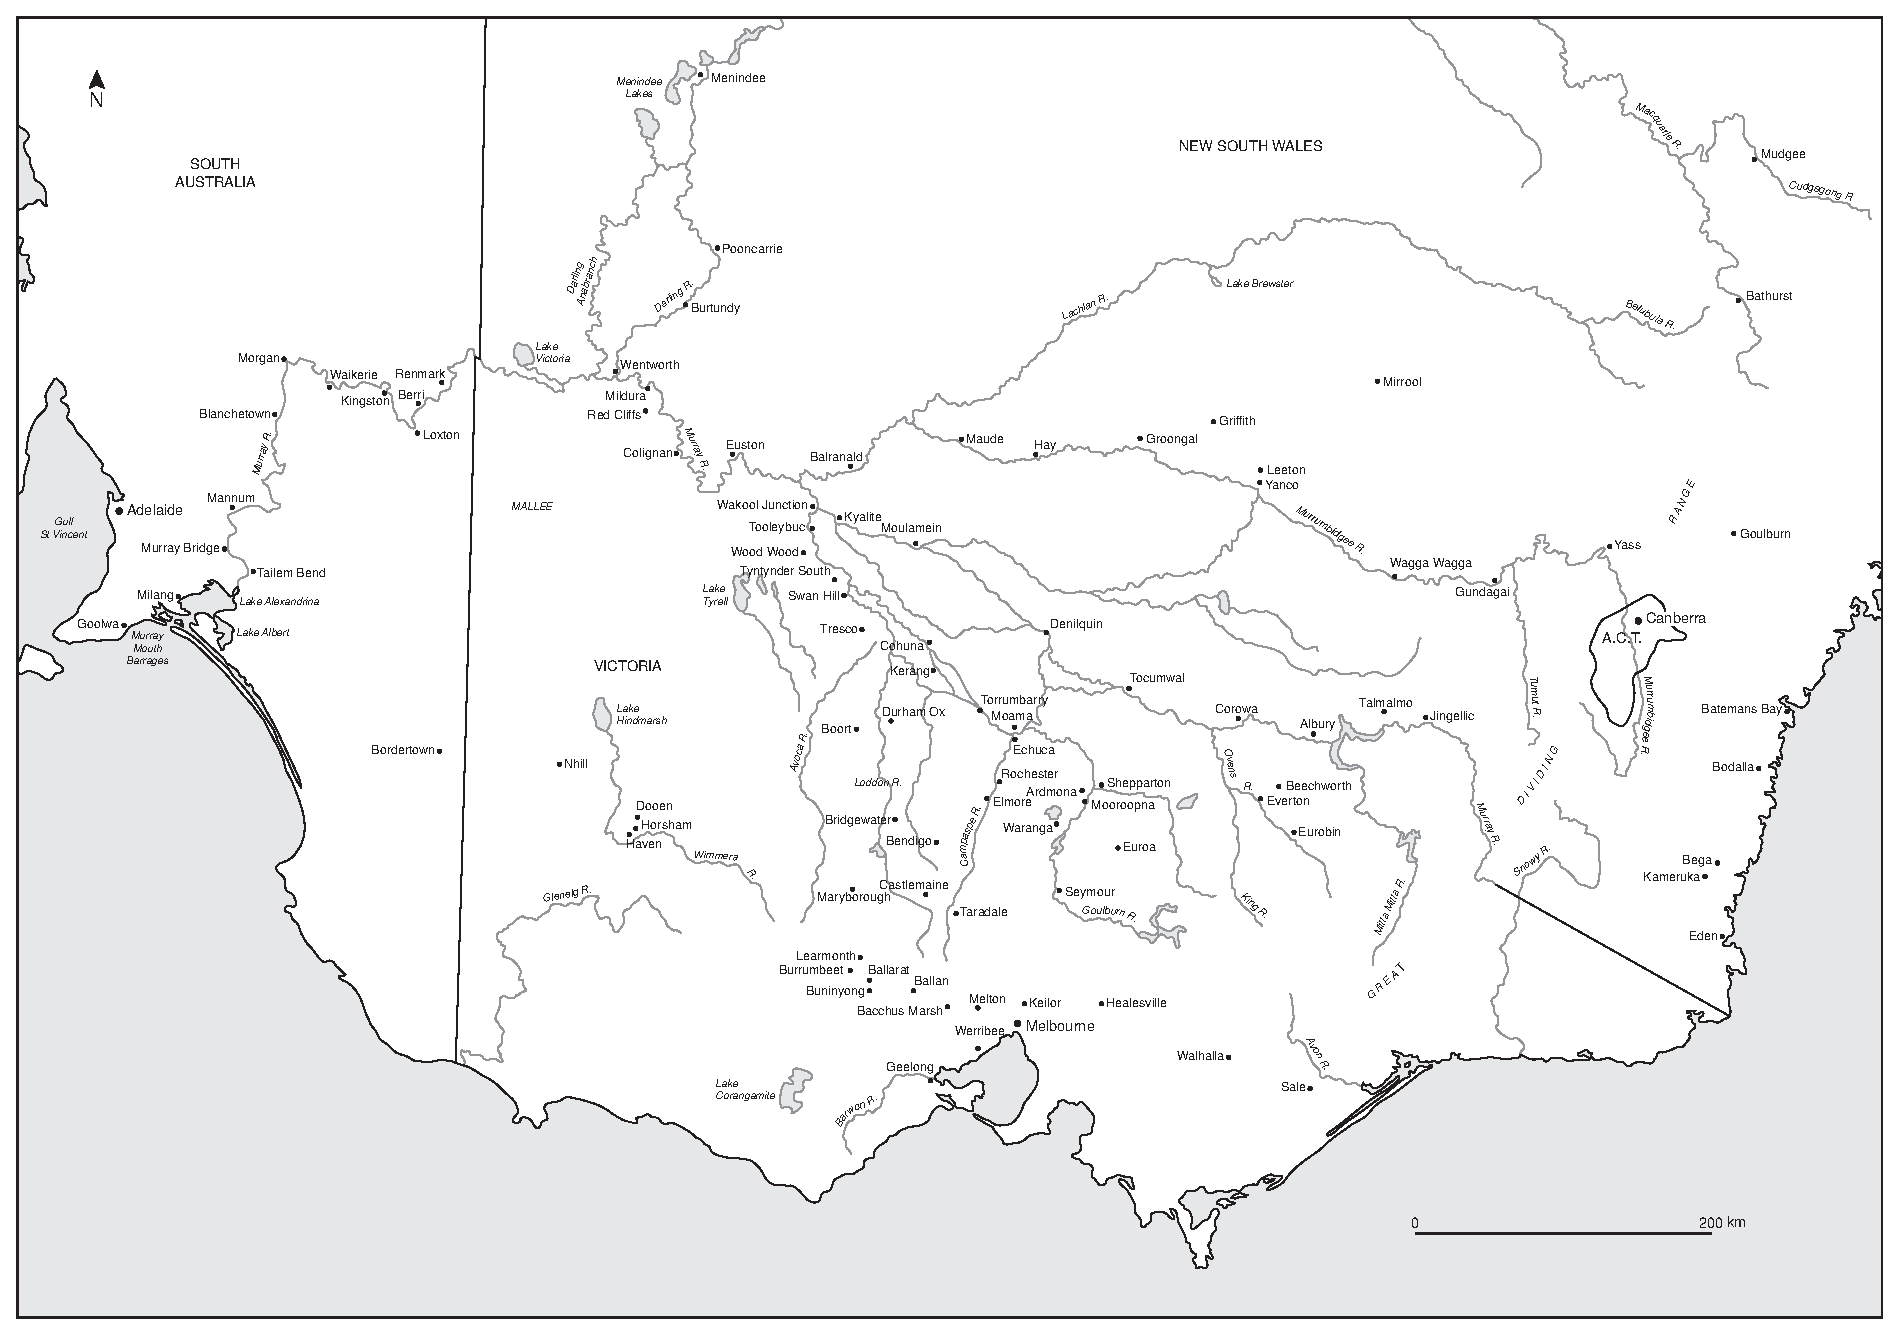
\includegraphics[bb=0 0 448 626,clip,width=1.123\textwidth]
{Figures/NSW_DOUBLE_PAGE.eps}}
\end{pspicture}
\newpage

\begin{pspicture}(0,0)(120mm,190mm)
\rput(48mm,96.2mm){
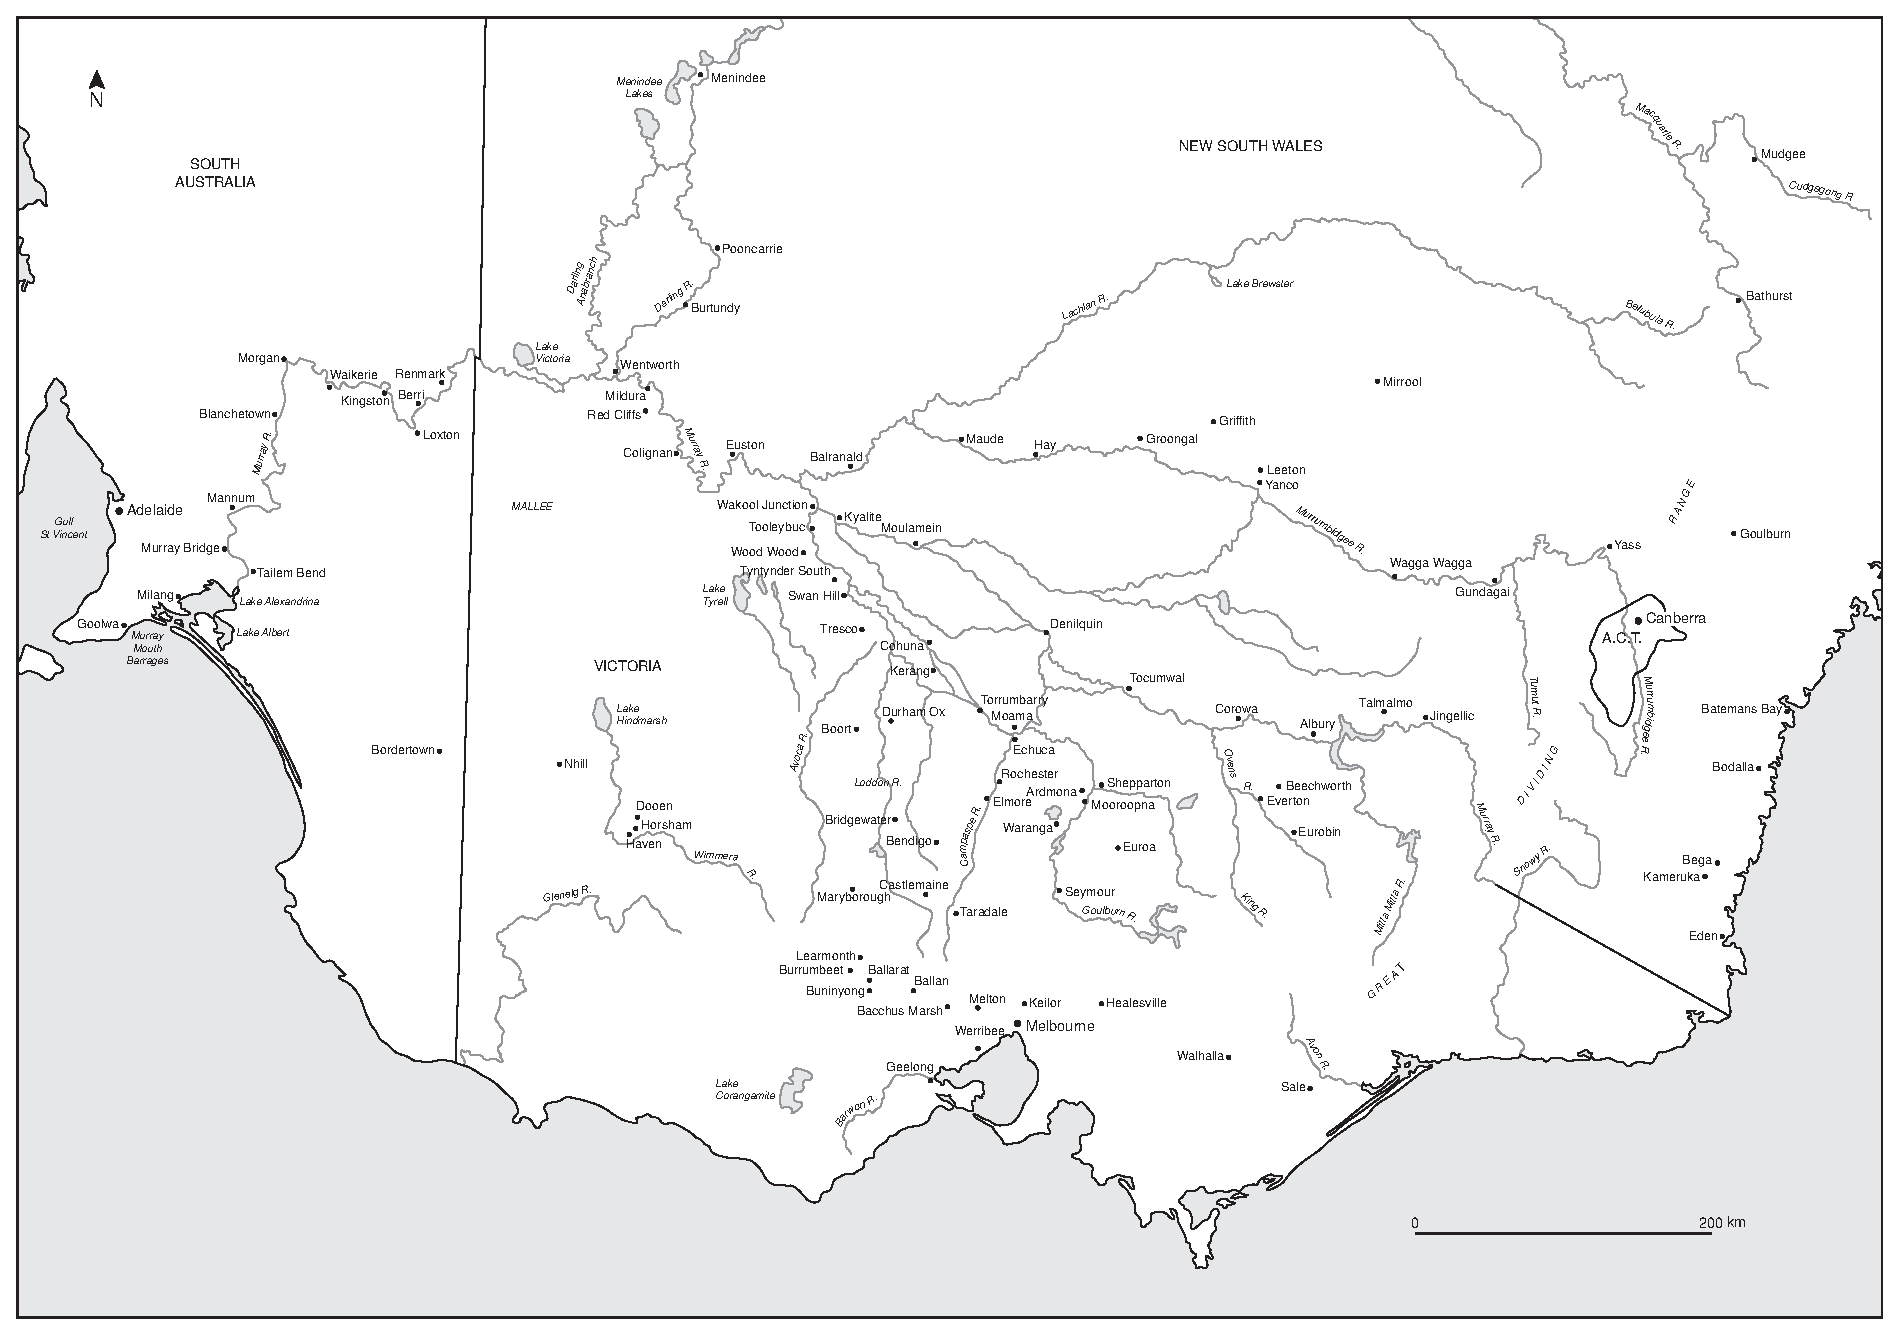
\includegraphics[bb=449 0 896 626,clip,width=1.123\textwidth]
{Figures/NSW_DOUBLE_PAGE.eps}}
\end{pspicture}
\vspace*{\fill}
\begin{center}
\sffamily
\textit{Rivers and sites of early irrigation in South-Eastern Australia}
\end{center}
\newpage

\begin{pspicture}(0,0)(120mm,190mm)
\rput(55.5mm,96.2mm){
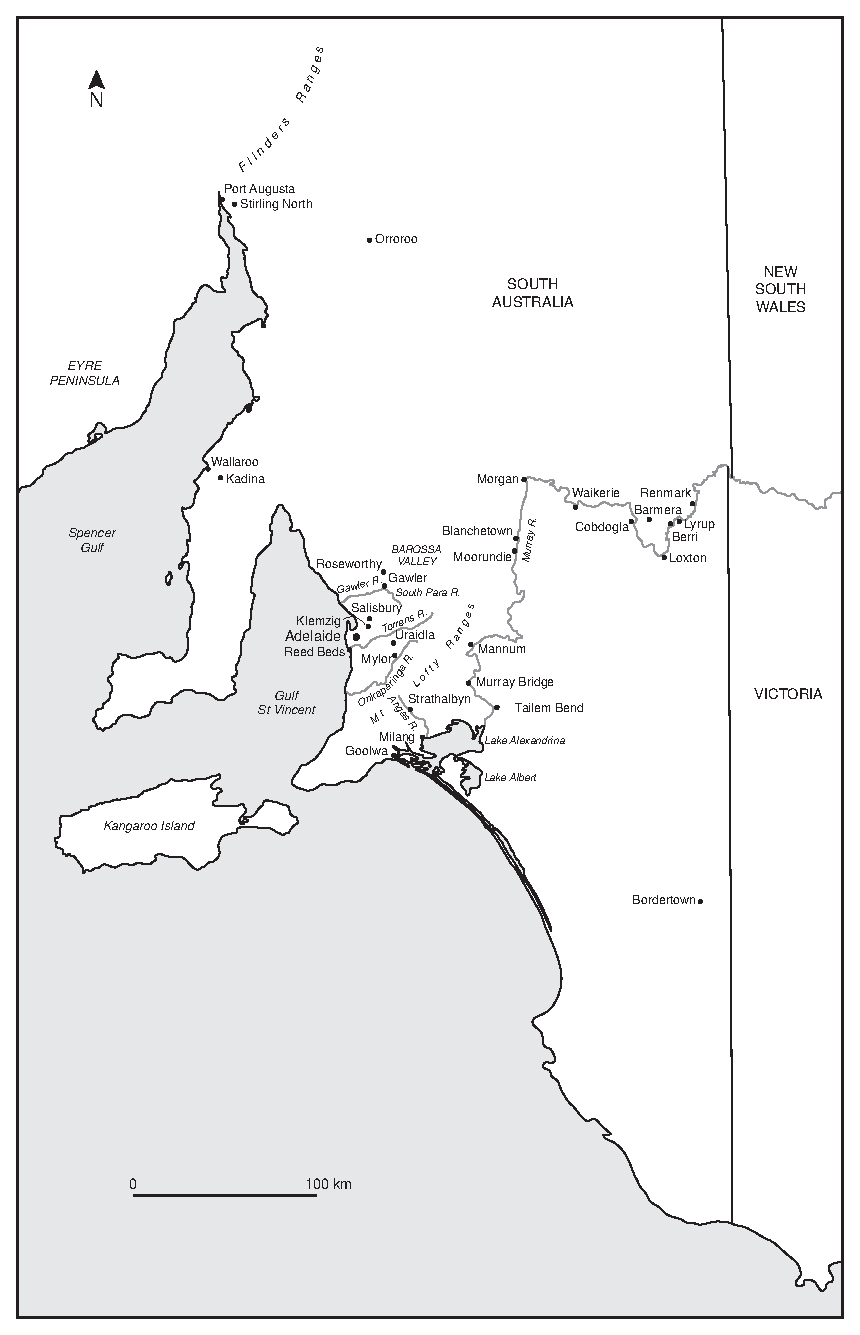
\includegraphics[width=\textwidth]{Figures/South_Australia.eps}}
\end{pspicture}
\vspace*{\fill}
\begin{center}
\sffamily
\textit{Rivers and sites of early irrigation in the Adelaide Region}
\end{center}
\newpage

\begin{pspicture}(0,0)(120mm,190mm)
\rput(55.5mm,96.2mm){
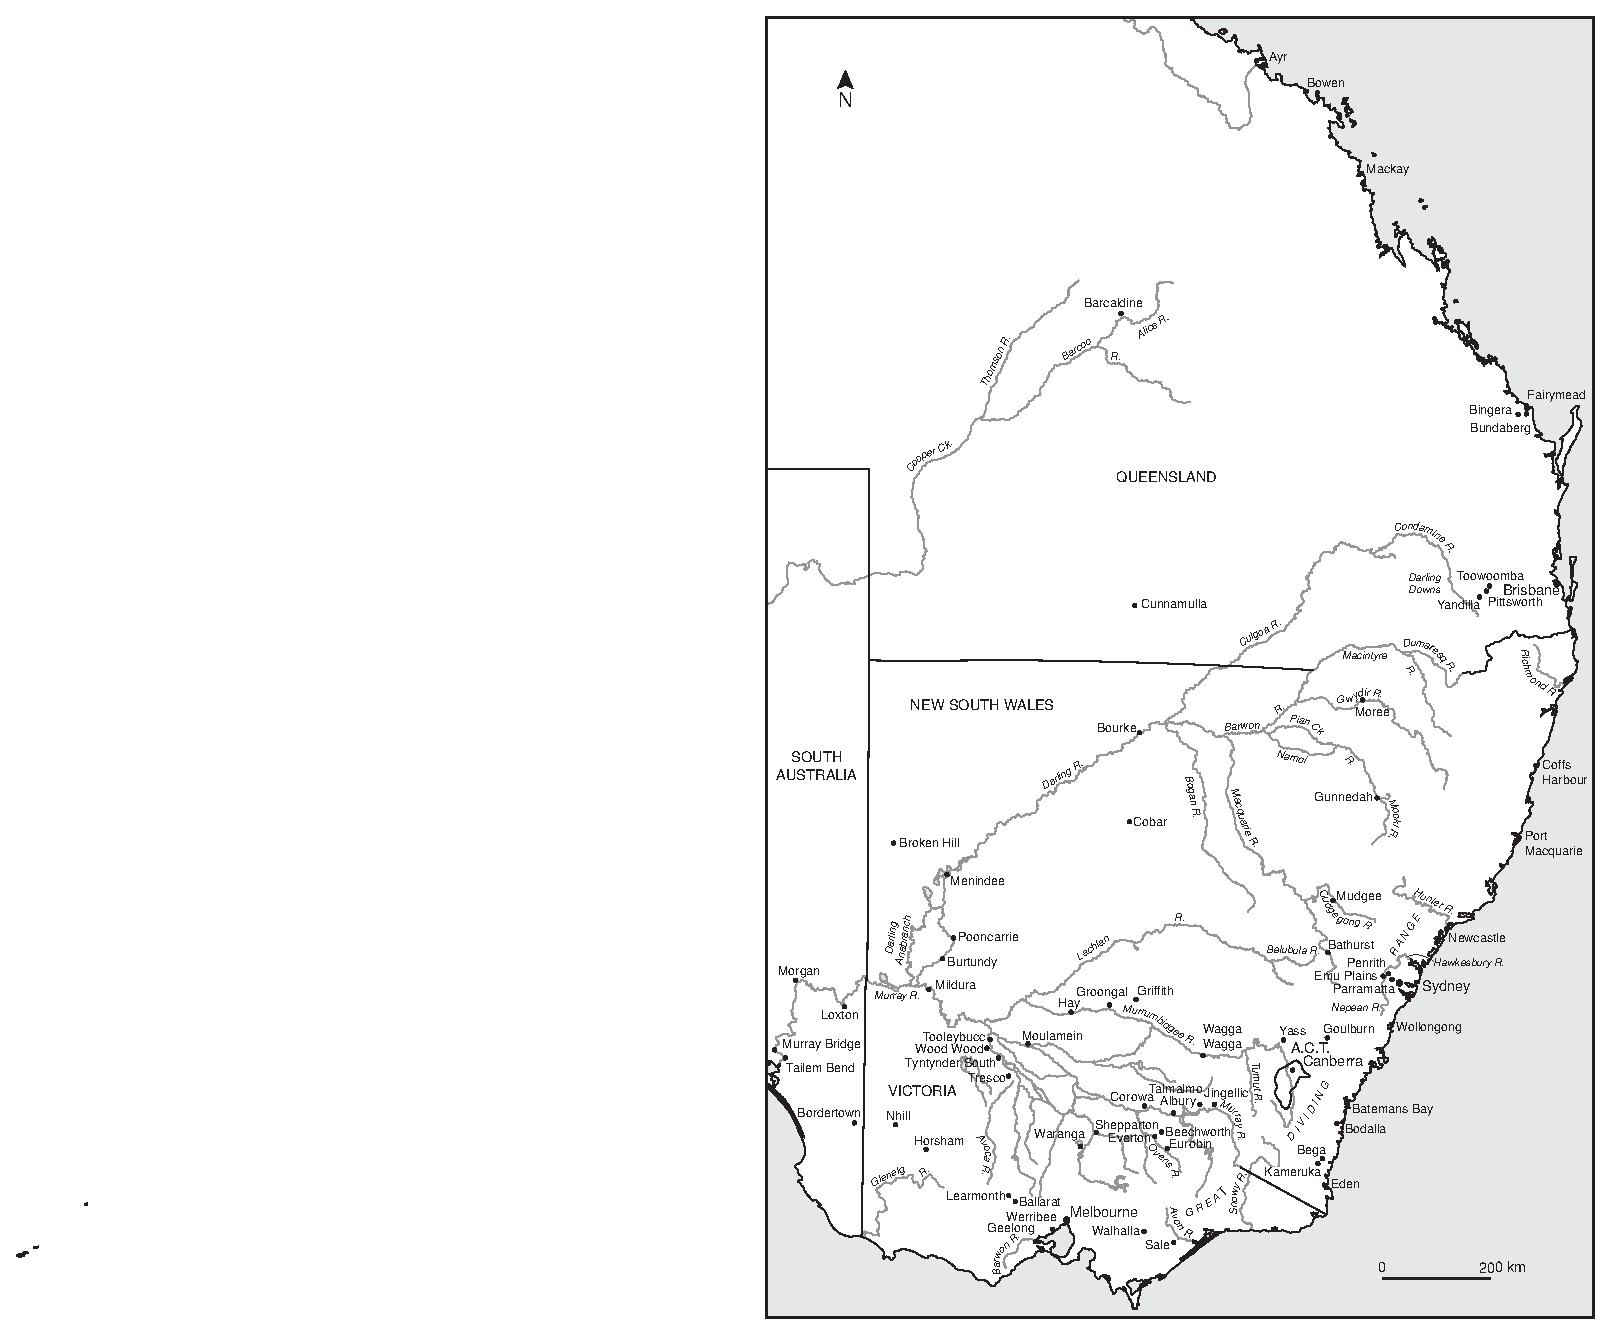
\includegraphics[width=\textwidth]{Figures/NSW_VIC.eps}}
\end{pspicture}
\vspace*{\fill}
\begin{center}
\sffamily
\textit{Rivers and sites of early irrigation in Eastern Australia}
\end{center}
\newpage

\begin{pspicture}(0,0)(120mm,190mm)
\rput(55.5mm,96.2mm){
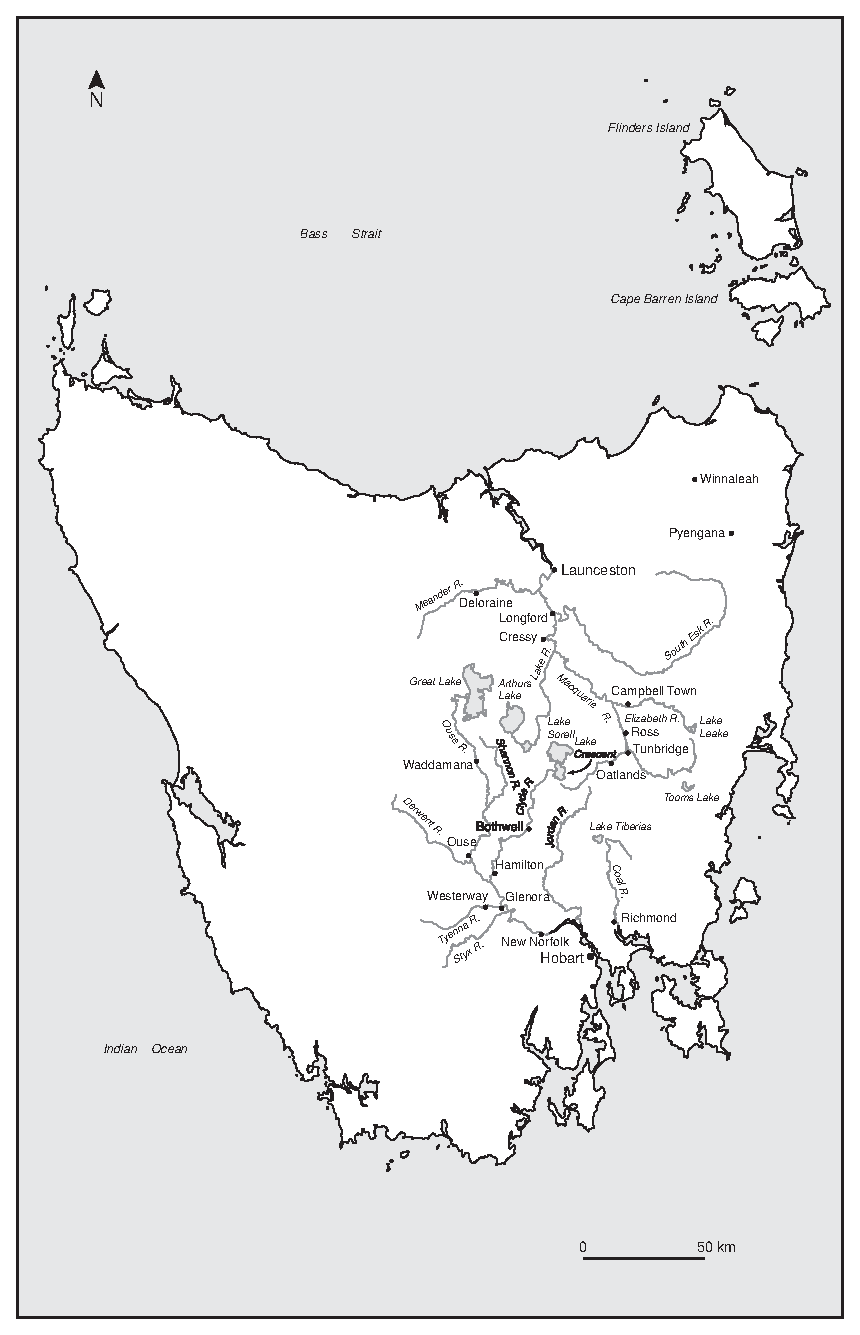
\includegraphics[width=\textwidth]{Figures/Tasmania.eps}}
\end{pspicture}
\vspace*{\fill}
\begin{center}
\sffamily
\textit{Rivers and sites of early irrigation in Tasmania}
\end{center}
